\subsection{All \hst Systems}

Below we present and briefly discuss the rest of the systems observed by our \hst program.
For each system, unless spectroscopic redshift is available, the photometric redshifts are form \citet{zhou2020a}.
We provide spectroscopic redshifts for the lensed sources whenever available.

All were confirmed to be strong lenses by \hst.
About half of them have a group/small cluster as the main lens 
A number of these systems show multiple sets of arcs.
The \hst images shown in the section are from WFC3 F140W observations, drizzled to 0.065$\twopr$.

\subsubsection{\href{https://www.legacysurvey.org/viewer/?ra=23.6765&dec=4.5639&layer=ls-dr9&pixscale=0.262&zoom=16}{DESI-023.6765+04.5639}}

The main lens in this system (Figure~\ref{fig:desi023}) appears to be the brightest galaxy in a small cluster or a group, with $z_{d, phot} = 0.553\pm0.014$
There are two large blue arcs visible in the LS image, with slightly different colors as well as different relative locations of star forming ``knots''. 
Thus it is likely that these two correspond to two different sources.
The \hst NIR F140W image further reveals an additional arc near the western edge of the cutout.

\begin{minipage}{\linewidth}
\makebox[\linewidth]{
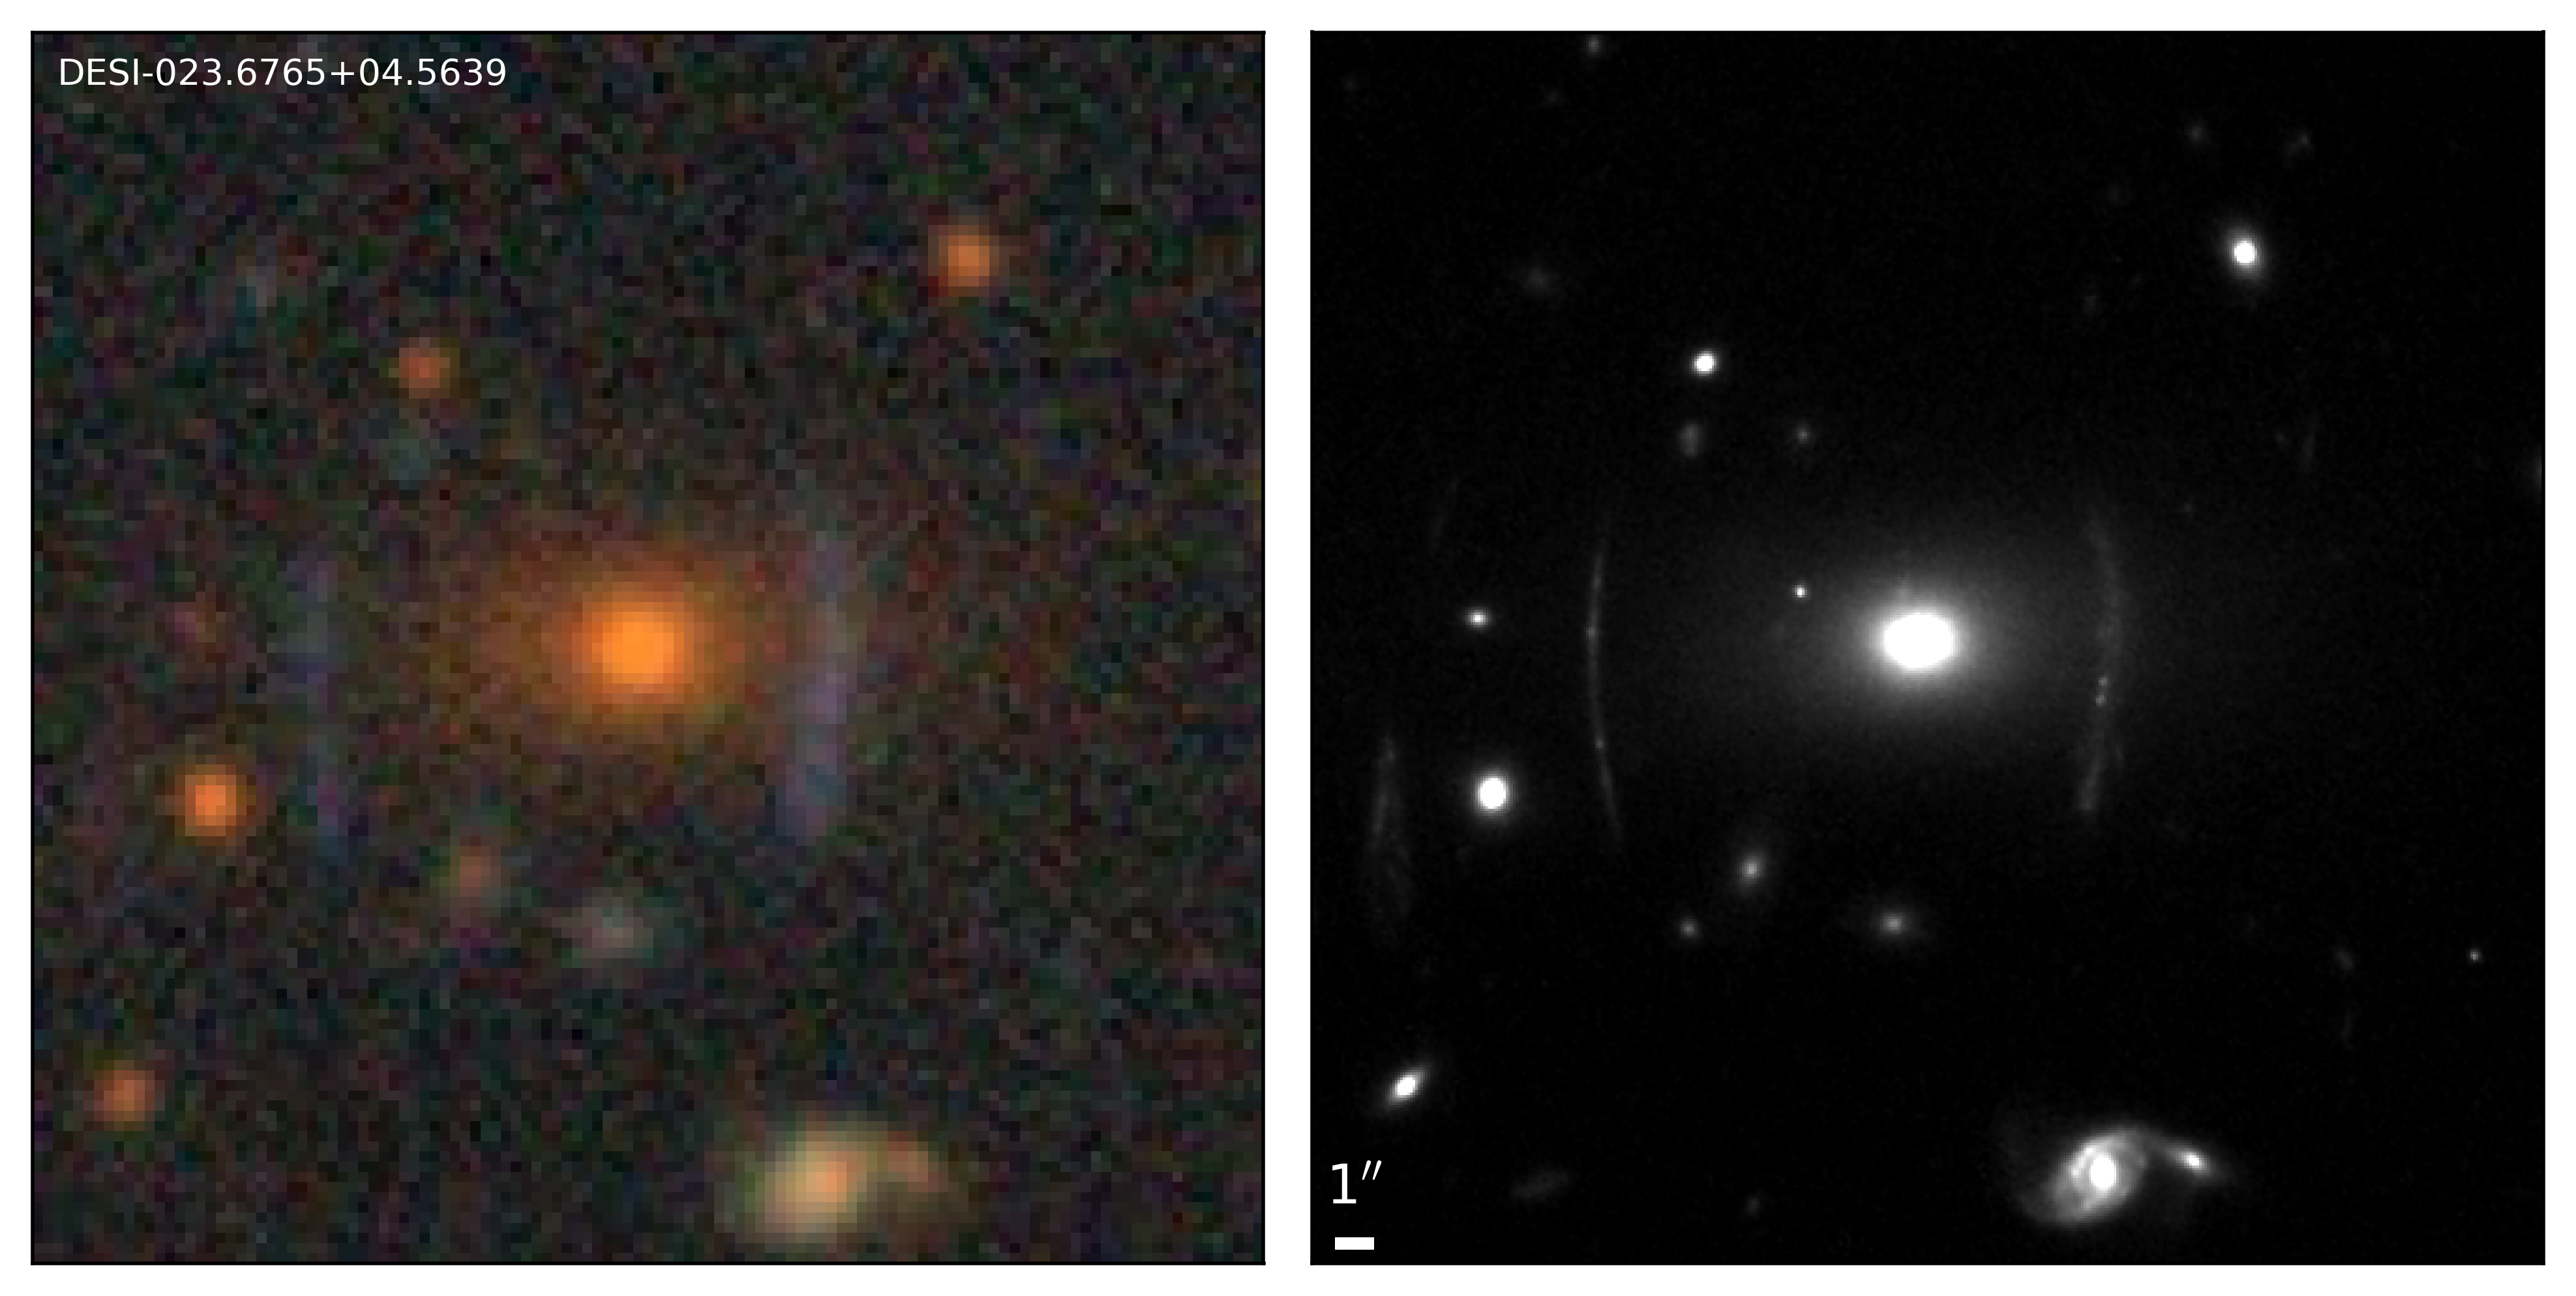
\includegraphics[keepaspectratio=true,scale=0.7]{figs/DESI-023_6765+04_5639.png}}
\captionof{figure}{DESI-023.6765+04.5639. 
On the left the $grz$ image from the DESI Legacy Surveys and the \hst F140W is shown on the right.
North is up and east to the left. This arrangement and this compass apply to all images in this section.
}
\label{fig:desi023}
\end{minipage}

\clearpage
\subsubsection{\href{https://www.legacysurvey.org/viewer/?ra=025.4848&dec=+30.7585&layer=ls-dr9&pixscale=0.262&zoom=16}{DESI-025.4848+30.7585}}

This is a galaxy-scale lens with at least two sources, with $z_d = 0.524$ from SDSS, which is further confirmed by DESI.
% $z_{d, phot} = 0.585\pm0.030$.
There is a hint of a blue lensed arc to the SW of the elliptical galaxy (Figure~\ref{fig:desi025}).
This was confirmed in the \hst image.
DESI provides the redshift for this source ($z_{s, 2} = 1.2223$; Huang et al. in prep).
Much closer to the lens than this source, there appear to be two arc-like structure.
\citet{talbot2021a} analyzed the lens spectrum closely and found evidence for a lensed source in the same SDSS fiber, and determined its redshift to be $z_{s, 1} = 1.216$, which must belong to one of these two.
 

\begin{minipage}{\linewidth}
\makebox[\linewidth]{
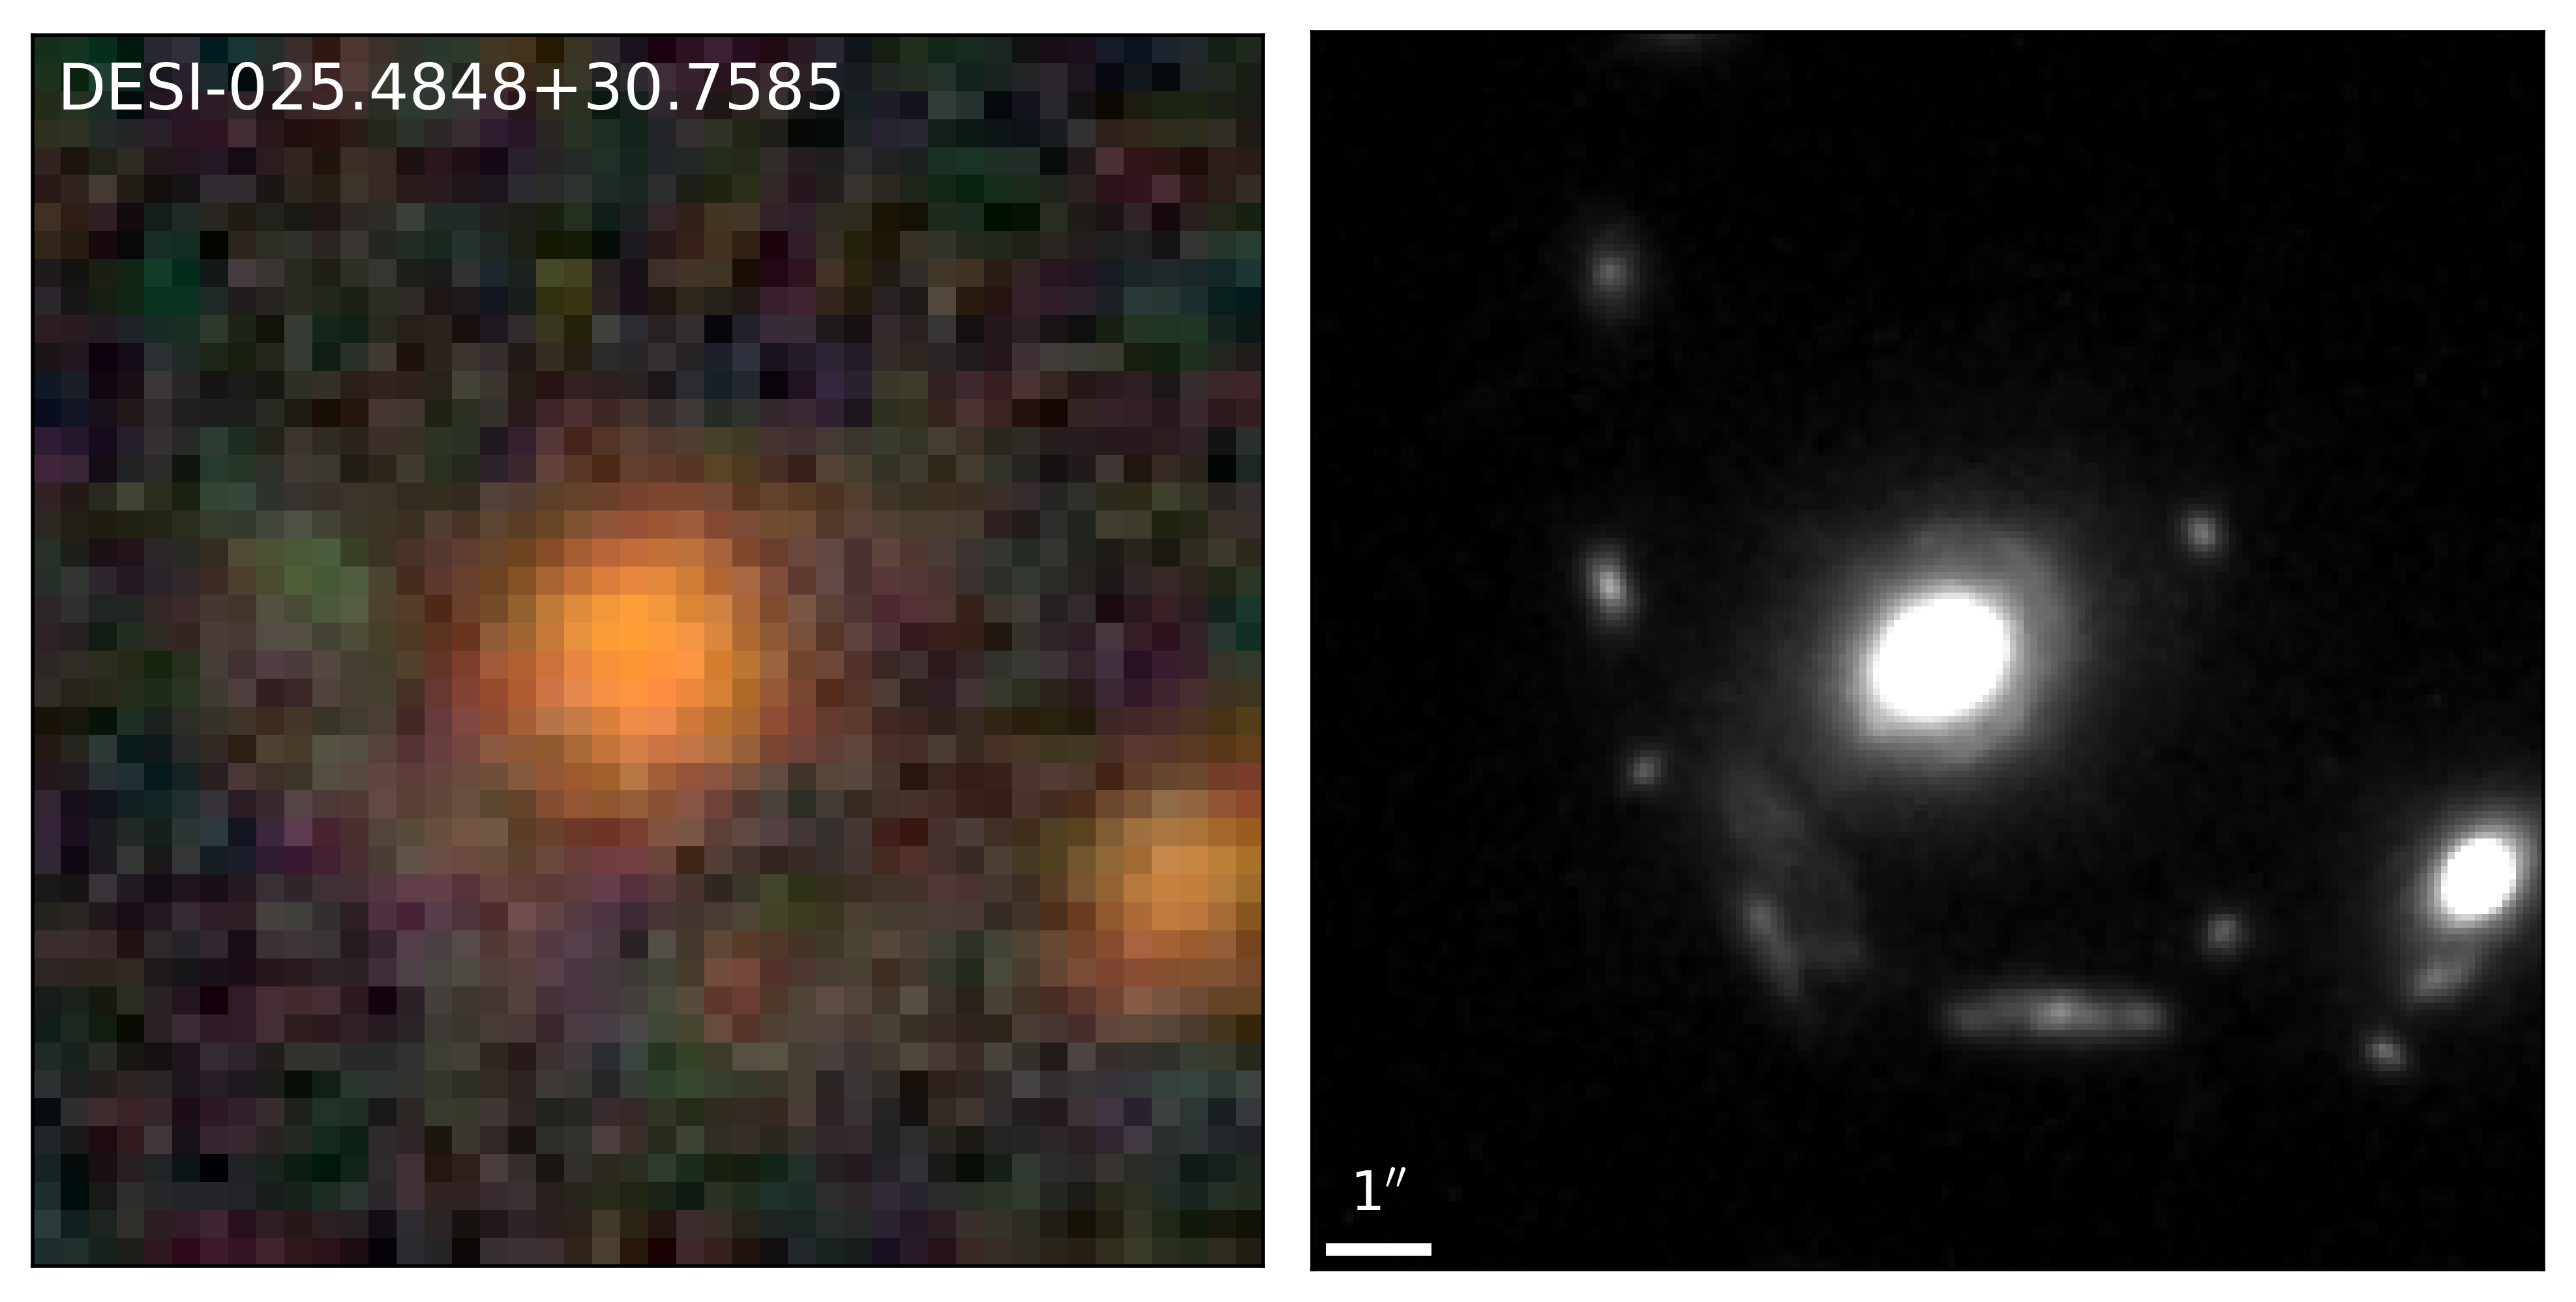
\includegraphics[keepaspectratio=true,scale=0.7]{figs/DESI-025_4848+30_7585.png}}
\captionof{figure}{DESI-023.6765+04.5639. 
For the arrangement of this figure, see the caption of Figure~\ref{fig:desi023}.}
\label{fig:desi025}
\end{minipage}

\subsubsection{\href{https://www.legacysurvey.org/viewer/?ra=186.4028&dec=-07.4188&layer=ls-dr9&pixscale=0.262&zoom=16}{DESI-186.4028-07.4188}}

% source spectrum: https://www.legacysurvey.org/viewer-desi/desi-spectrum/dr1/targetid2349764821647361

This is also one of the less obvious systems. 
\hst showed two arclets on either side of the elliptical galaxy.
DESI has further provided spectroscopic confirmation, 
with $z_d = 0.405$ and $z_s = 1.0838$ for the arclet to the NE of the lens.


\subsubsection{\href{https://www.legacysurvey.org/viewer/?ra=023.0157&dec=-16.0040&layer=ls-dr9&pixscale=0.262&zoom=16}{DESI-023.0157-16.0040}}
% source: https://www.legacysurvey.org/viewer-desi/desi-spectrum/daily/targetid2789365738635264

In H21, Human score: 3 (Grade B), probability: 0.98

$z_d$ = $0.492\pm0.047$ from SDSS
From DESI: $z_s$ = 1.5818


\subsubsection{DESI-030.4360-27.6617}

Another single-galaxy system

\begin{minipage}{\linewidth}
\makebox[\linewidth]{
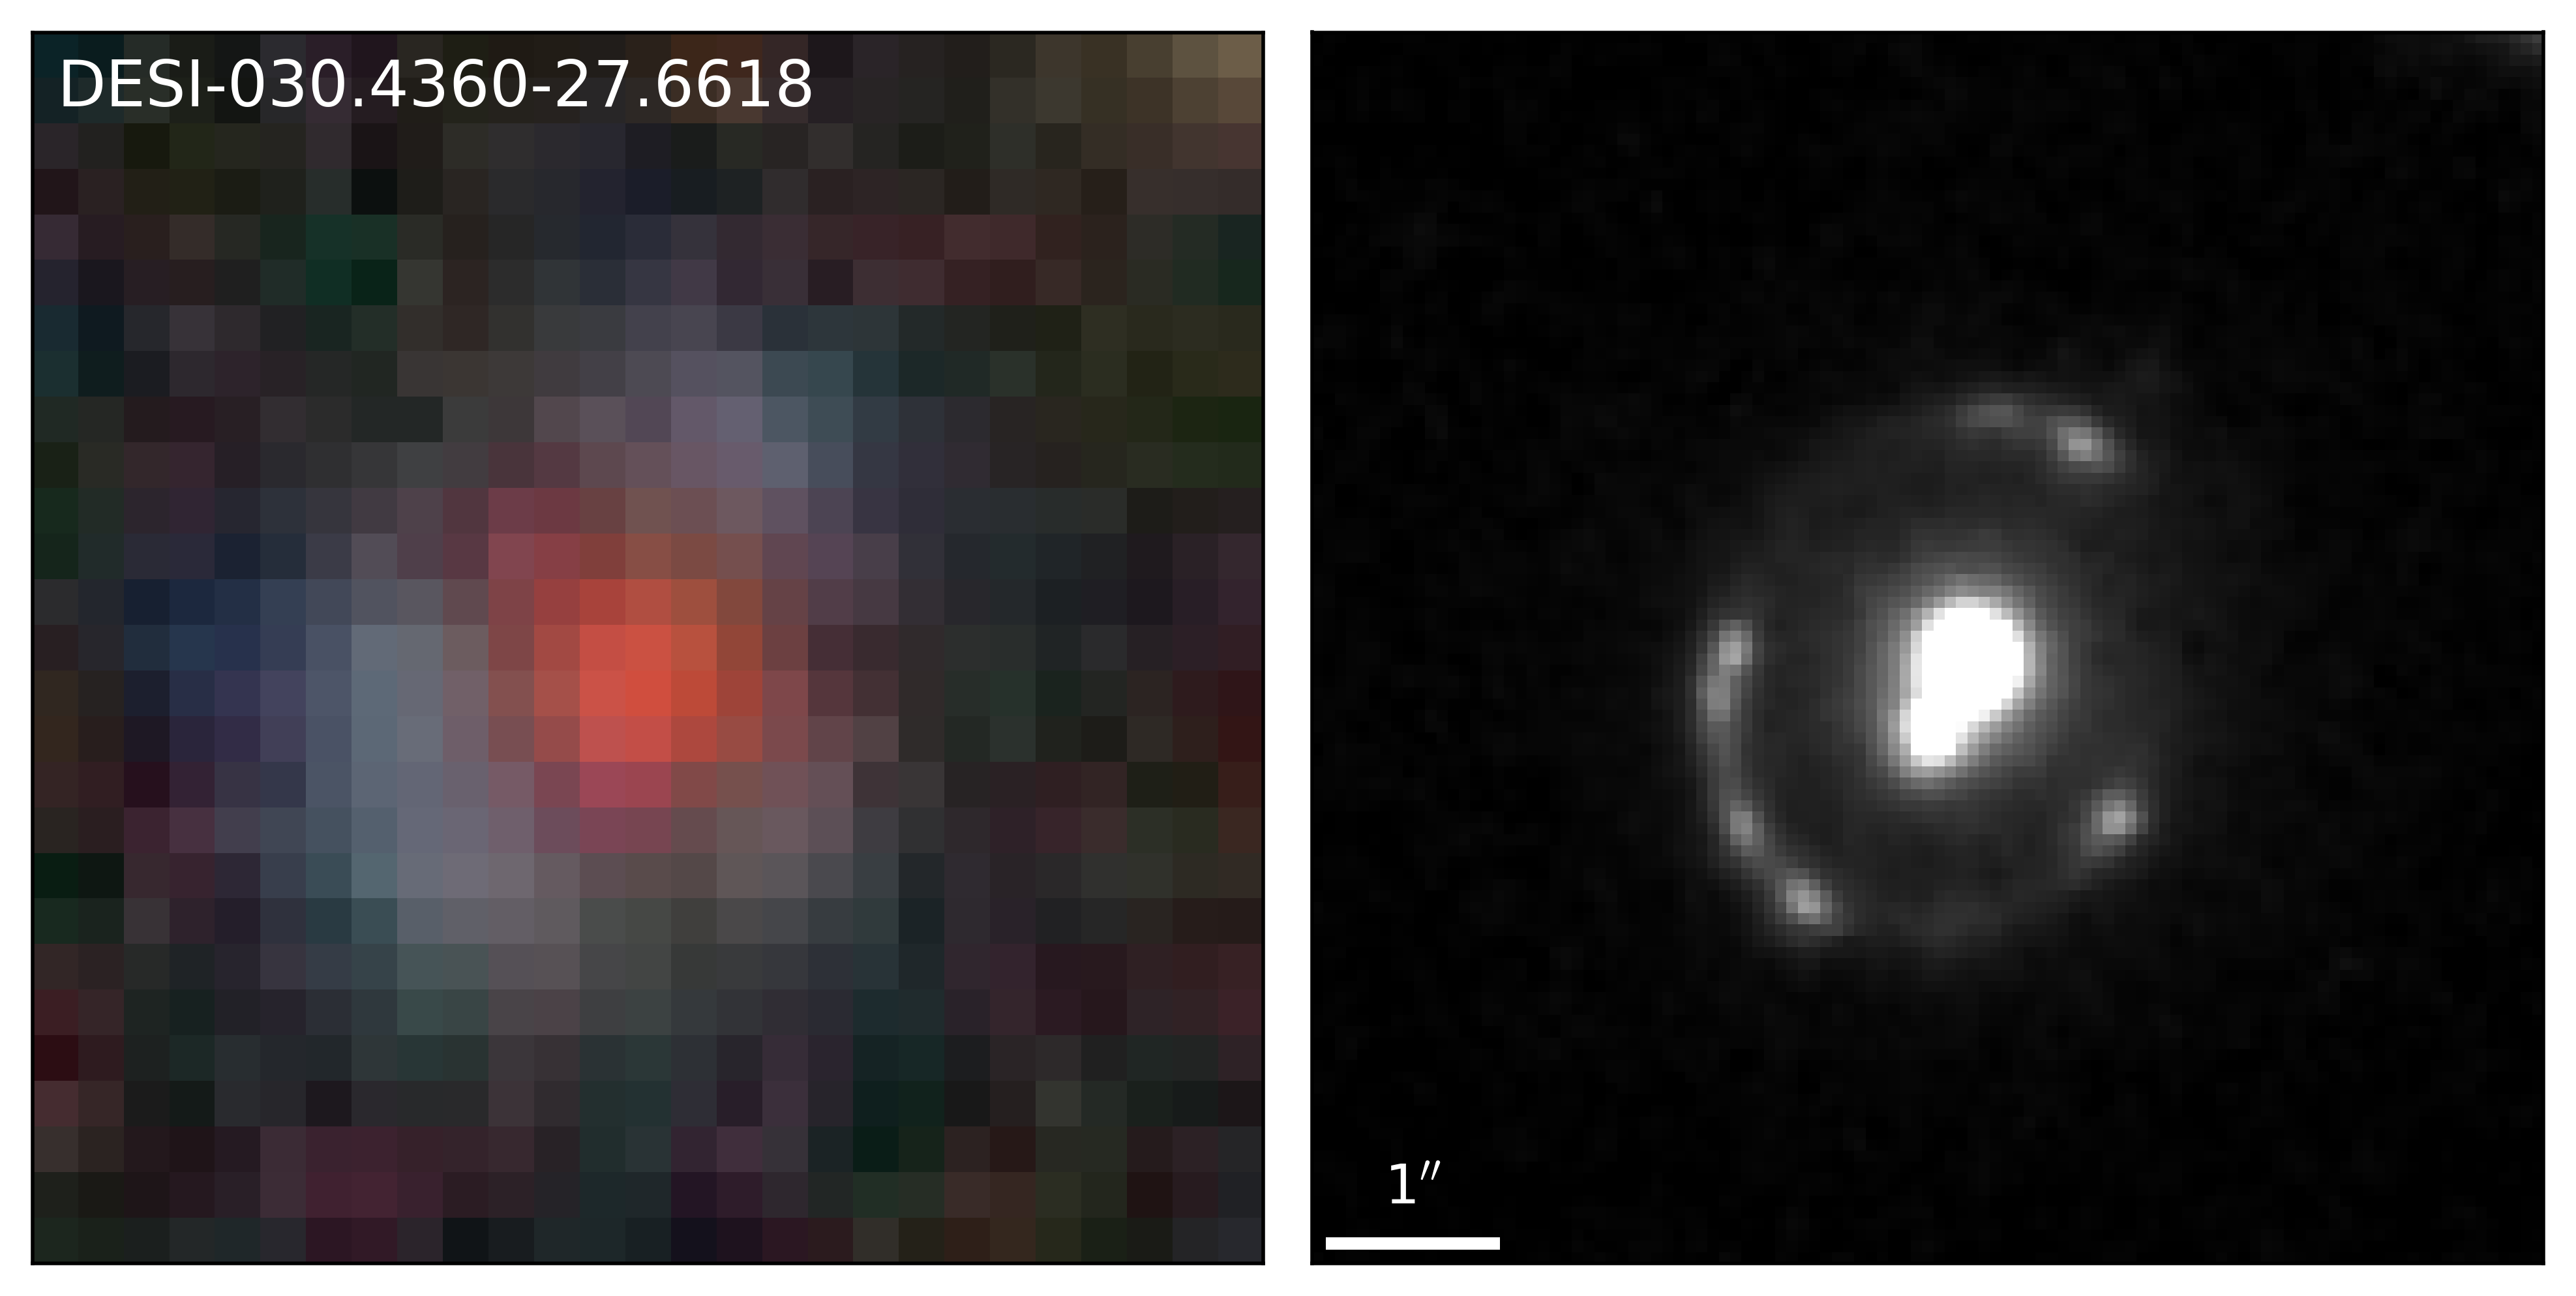
\includegraphics[keepaspectratio=true,scale=0.7]{figs/DESI-030_4360-27_6617.png}}
\captionof{figure}{DESI-023.6765+04.5639. 
For the arrangement of this figure, see the caption of Figure~\ref{fig:desi023}.}
\label{fig:desi030}
\end{minipage}

% \begin{minipage}{\linewidth}
% \makebox[\linewidth]{
%   \includegraphics[keepaspectratio=true,scale=0.75]{figs/gal-lenses-LS.pdf}}
% \makebox[\linewidth]{
% \includegraphics[keepaspectratio=true,scale=0.742]{figs/gal-lenses-HST.pdf}}
% \captionof{figure}{{\color{red} A Bolton suggestion: put LS and HST figures side-by-side}
% The 26 systems with a single galaxy as the main lens observed by the \hst SNAP program 15867. 
% All were confirmed to be strong lenses by \hst with arc(s) in each clearly revealed.
% The first one at top left has the faintest arcs (see text).
% The top panel shows the Legacy Surveys images for these systems (discovery images),
% in order of increasing Einstein radii,
% with North up, East to the left. 
% The naming convention is R.A. and decl. in decimal format.
% The bottom panel shows the \hst WFC3 F140W images for the same systems, drizzled to 0.065$\twopr$.
% There are a number of striking systems (see text).
% \S~\ref{sec:lens-model} presents the lens model for DESI-165.4754=06.0423.}
% \label{fig:gal-lenses}
% \end{minipage}

\clearpage
\subsubsection{DESI-189.5370+15.0309}
In Figure~\ref{fig:desi189} shows DESI-189.5370+15.0309.
It shows a small group of galaxies with similar red colors.
Around the brightest group galaxy, there appears to be a large reddish arc. 
To the SW to the brightest group galaxy, there is a group member.
Approximately along the line connecting these two galaxies,
in the diametrically opposite direction, at $\sim 13.5''$,
there is a small arc with a similar color.
These arcs are revealed in the \hst image to have very similar spiral structure, almost certainly two images of the same background source galaxy (two ``half cinnamon buns'').
\begin{minipage}{\linewidth}
\makebox[\linewidth]{
  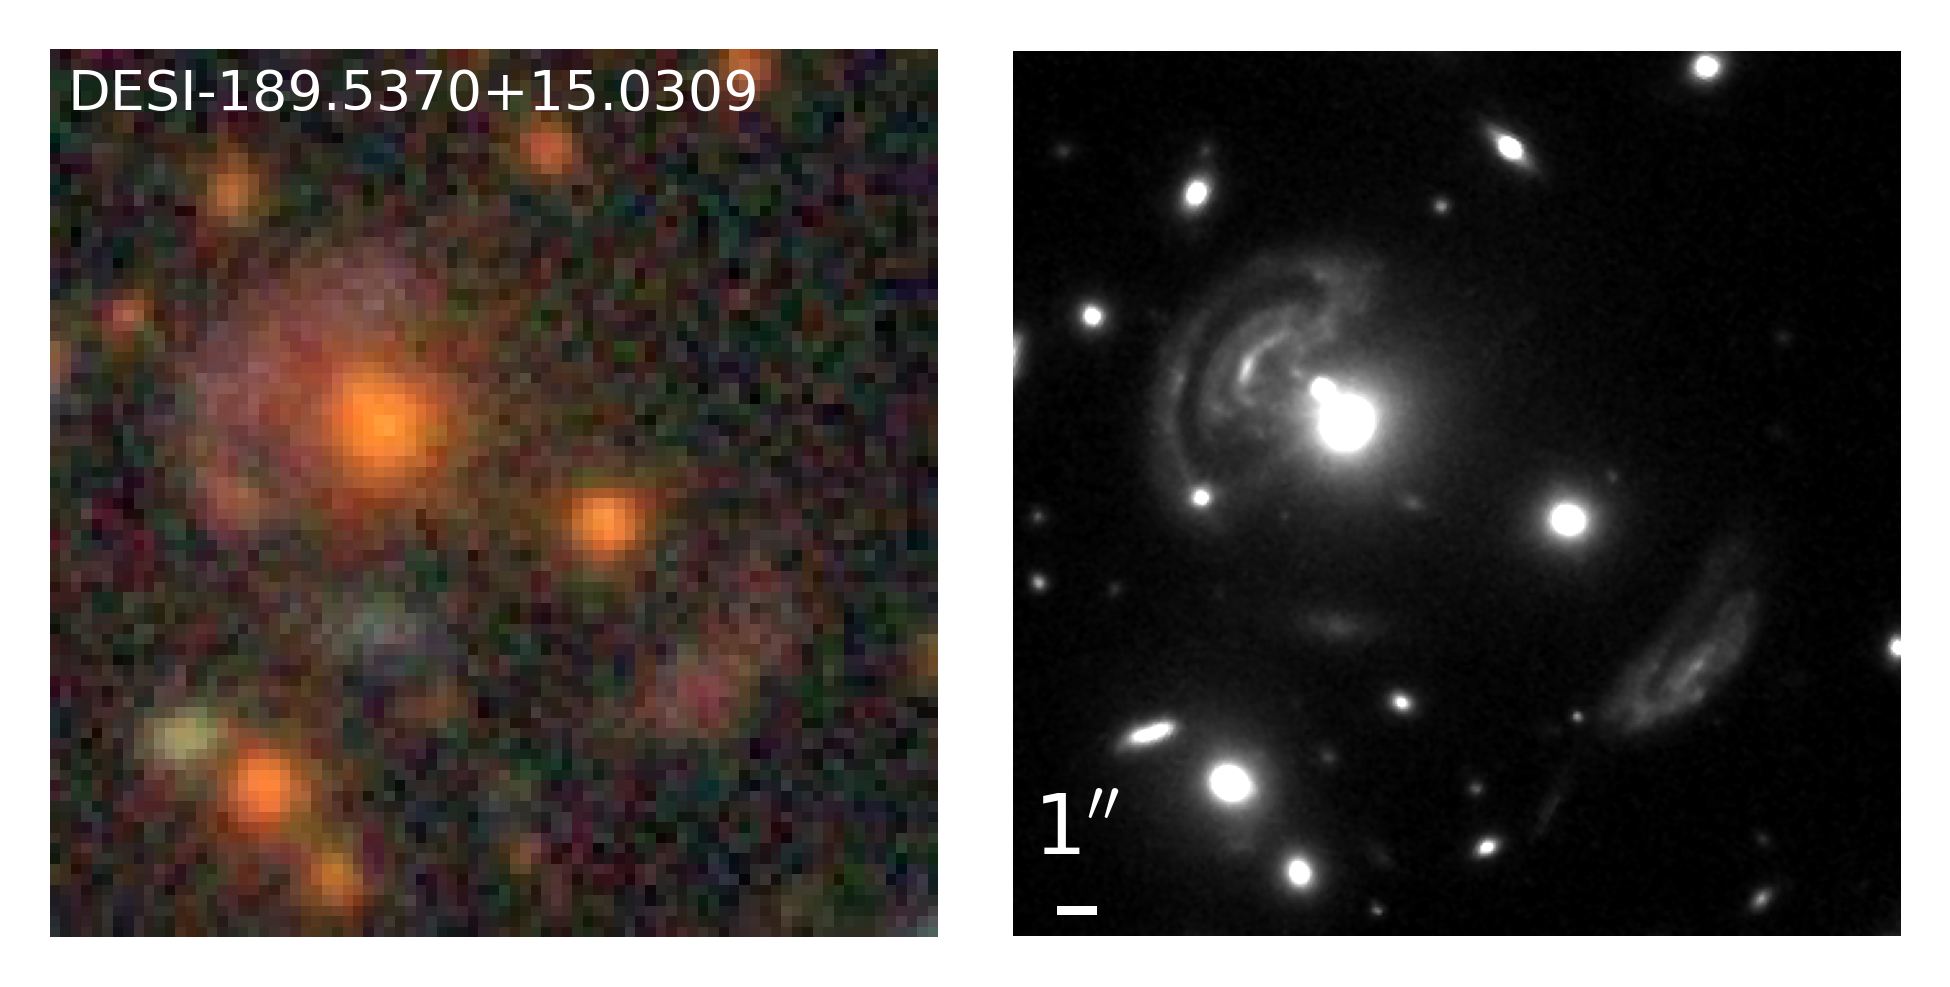
\includegraphics[keepaspectratio=true,scale=0.9]{figs/DESI-189.png}}
% \makebox[\linewidth]{
  % \includegraphics[keepaspectratio=true,scale=0.76]{figs/group-lenses-HST.pdf}}
\captionof{figure}{
DESI-189.5370+15.0309.
}
\label{fig:desi189}
\end{minipage}

% \begin{figure}
% \includegraphics[]{figs\DESI-023.6765+04.5639.png}
% \end{figure}
